\documentclass{article}
\usepackage[utf8]{inputenc}
\usepackage[spanish]{babel}
\usepackage{vmargin}
\usepackage{tikz}
\usepackage{tikz-uml}
\usepackage[hidelinks]{hyperref}
\usepackage{listings}
\usepackage{graphicx}
\graphicspath{ {img/} }

\usepackage{caption}
\usepackage{subcaption}
\DeclareCaptionLabelFormat{cont}{#1~#2\alph{ContinuedFloat}}
\captionsetup[ContinuedFloat]{labelformat=cont}





\definecolor{primaryKey}{HTML}{E5BD05}
\definecolor{foreignKey}{HTML}{CC5A0B}
\definecolor{sentence}{HTML}{0B6C9D}
\definecolor{numberSQL}{HTML}{E57D01}


\setpapersize{A4}
\setlength{\parindent}{0px}

\title{\textbf{\underline{PROYECTO FULL-STACK}}}
\author{Néstor Batista Díaz }
\date{}

\usetikzlibrary{positioning,shapes.multipart,shapes,er}

\begin{document}
\large
\maketitle
\vspace{20mm}
\begin{figure}[h]
    \centering
    
\includegraphics[scale=0.5]{logoIES}
\end{figure}
\newpage

\newpage

\setcounter{tocdepth}{2}
\tableofcontents

\newpage

\section{Introducción}
\quad Este proyecto se desarrollara para la empresa Tandem Enterprise.\\
El proyecto propuesto por la empresa consiste en implementar una idea de comercio orientada a los productos canarios. En la aplicación se podrán ver, crear, actualizar y eliminar productos de procedencia canaria.\\También habrá usuarios, que se tendrán que registrar para poder realizar un pedido. Si un usuario no se ha registrado o no ha iniciado sesión solo podra ver los productos que hay disponibles, pero no podra realizar ningún pedido.\\ Al usuario se le pedira los datos necesarios para poder realizar la compra(nombre, email, contraseña y direccion).\\
Por ahora, la empresa nos ha pedido que lleguemos hasta la pantalla de compra, asi que no se pediran datos relacionados con la cuenta bancaria ni con targetas de credito o debito.
\section{Modelo de Datos}
\quad Aqui se mostrara como esta organizada la base de datos del proyecto.
\subsection{Descripción}
\begin{itemize}
    \item \textbf{Entidades} \\\\
En la base de datos tendra que tener los siguientes campos:
\begin{itemize}
    \item Usuarios, que tendra una clave, un nombre, apellido, email, nombre de usuario, contraseña y tambien se tendra que saber si es administrador o no.
    \item Direccion del usuario, se almacenara la direccion de cada usuario, y se devera tener, una clave, la calle, numero, codigo postal, localidad, provincia y pais.
    \item Pedidos, se almacenara una clave, la fecha y estado. 
    \item Productos, se almacenara una clave, un nombre, la descripción, precio, porcentaje de impuestos, categoria, saber si esta disponible y una imagen del producto.
\end{itemize}
\item \textbf{Relaciones} 
\begin{itemize}
    \item Un usuario solo puede tener una dirección y una dirección pertenece a un solo usuario. 
    \item Un usuario puede hacer varios pedidos, pero un pedido pertenece solo a un usuario.
    \item Un pedido puede tener varios productos y un producto puede estar en varios pedidos.
\end{itemize}
\end{itemize}
\subsection{Diagrama E/R}
\tikzset{basic/.style={
        draw,
        rectangle split,
        rectangle split parts=2,
        rectangle split part fill={violet!50,white},
        minimum width=2.5cm,
        text width=2cm,
        align=left
    },
    Diamond/.style={ diamond, 
                        draw, 
                        shape aspect=2, 
                        inner sep = 2pt,
                        text centered,
                        fill=violet!20!white
                      }}
\begin{tikzpicture}
\node[basic] (products) {products
\nodepart{second}
\underline{id}\\
name\\
description\\
price\\
tax\_rate\\
image\\
category\\
availability};

\node[basic,right=5cm of products] 
(orders)
{orders
\nodepart{second}
\underline{id}\\
date\\
status};

\node[basic,below=5cm of orders] 
(users)
{users
\nodepart{second}
\underline{id}\\
name\\
last\_name\\
userName\\
email\\
password\\
isAdmin};

\node[basic,left=5cm of users] 
(address)
{address
\nodepart{second}
\underline{id}\\
street\\
number\\
zip\_code\\
location\\
province\\
country};


\draw (products) -- (orders) node[midway,Diamond](contiene){contain}
child[grow=up,level distance=3cm] {node[attribute] {timestamp}};
\path [align=center, below](contiene) edge node {(\(1\),\(n\))} (products)
    edge node {(\(1\),\(n\))}	(orders);
\node[below = 2mm of contiene]{N:M};

\draw (orders) -- (users) node[midway,Diamond](hace){make}
child[grow=right,level distance=3cm] {node[attribute] {timestamp}};
\path [align=center, right](hace) edge node {(\(0\),\(n\))} (orders)
    edge node {(\(1\),\(1\))}	(users);
\node[left = 2mm of hace]{1:N};

\draw (users) -- (address) node[midway,Diamond](tiene){have};
\path [align=center, below](tiene) edge node {(\(1\),\(1\))} (users)
    edge node {(\(1\),\(1\))}	(address);
\node[below = 2mm of tiene]{1:1};

\end{tikzpicture}

\subsection{Paso de E/R a Modelo relacional}
\quad Las palabras subrayadas son claves primarias y las que tienen asterisco son claves foraneas.\\
\textsc{Products} (\underline{\textbf{id}}, name, description, price,tax\_rate, image, category, availability).\\\\
\textsc{Order\_product} (\underline{\textbf{id\_product*}}, \underline{\textbf{id\_order*}}, timestamp).\\
\textbf{id\_product} es clave foranea de \textsc{products}.\\
\textbf{id\_order} es clave foranea de \textsc{orders}.\\\\
\textsc{Orders} (\underline{\textbf{id}}, date, status, timestamp, \textbf{id\_user*}).\\
\textbf{id\_user*} es clave foranea de \textsc{users}.\\\\
\textsc{Users} (\underline{\textbf{id}}, name, last\_name,userName, email, password, isAdmin, timestamp, \textbf{id\_address*}).\\
\textbf{id\_address} es clave foranea de \textsc{address}.\\\\
\textsc{Address} (\underline{\textbf{id}},street,number,zip\_code, location, province, country).

\subsection{Modelo Relacional}
\tikzset{basic2/.style={
        draw,
        rectangle split,
        rectangle split parts=2,
        rectangle split part fill={violet!50,white},
        minimum width=4cm,
        text width=5cm,
        align=left
    }}

\begin{tikzpicture}
\node[basic2](orderProduct){
order\_product
\nodepart{second}
\textcolor{primaryKey}{(PK)} \textcolor{foreignKey}{(FK)} id\_product INT\\
\textcolor{primaryKey}{(PK)} \textcolor{foreignKey}{(FK)} id\_order INT\\
timestamp TIMESTAMP
};

\node[basic2,below=5cm of orderProduct] (products) {products
\nodepart{second}
\textcolor{primaryKey}{(PK)} id INT\\
name STRING\\
description STRING\\
price FLOAT\\
tax\_rate FLOAT\\
image STRING\\
category STRING\\
availability BOOLEAN};



\node[basic2,right=5cm of orderProduct] 
(orders)
{orders
\nodepart{second}
\textcolor{primaryKey}{(PK)} id INT\\
date DATE\\
status STRING\\
timestamp TIMESTAMP\\
\textcolor{foreignKey}{(FK)} id\_user INT
};

\node[basic2,below=5cm of orders] 
(users)
{users
\nodepart{second}
\textcolor{primaryKey}{(PK)} id INT\\
name STRING\\
last\_name STRING\\
userName STRING\\
email STRING\\
password STRING\\
isAdmin BOOLEAN\\
timestamp  TIMESTAMP\\
\textcolor{foreignKey}{(FK)} id\_address INT};

\node[basic2,below=5cm of users] 
(address)
{address
\nodepart{second}
\textcolor{primaryKey}{(PK)} id INT\\
street STRING\\
number STRING\\
zip\_code INT\\
location STRING\\
province STRING\\
country STRING};


\draw (products) -- (orderProduct) node[midway](contiene1){};
\path [align=center, right](contiene1) edge node {(\(1\),\(1\))} (products)
    edge node {(\(1\),\(n\))}	(orderProduct);

\draw (orderProduct) -- (orders) node[midway](contiene2){};
\path [align=center, below](contiene2) edge node {(\(1\),\(n\))} (orderProduct)
   edge node {(\(1\),\(1\))}	(orders);

\draw (orders) -- (users)
node[midway](hay){};
\path [align=center, right](hay) edge node {(\(0\),\(n\))} (orders)
   edge node {(\(1\),\(1\))} (users);
   
\draw (users) -- (address)
node[midway](tiene){};
\path [align=center, right](tiene) edge node {(\(1\),\(1\))} (users)
   edge node {(\(1\),\(1\))} (address);

\end{tikzpicture}

\subsection{SQL}
\textsc{\textcolor{sentence}{drop database if exists}} db\_e\_commerce;\\
\textsc{\textcolor{sentence}{create database}} db\_e\_commerce;\\\\
\textsc{\textcolor{sentence}{use}} db\_e\_commerce;\\\\
\textsc{\textcolor{sentence}{drop table if exists}} products;\\
\textsc{\textcolor{sentence}{create table}} products (\\
\phantom{abc} id \textsc{\textcolor{sentence}{int primary key auto\_increment}},\\
\phantom{abc} name \textsc{\textcolor{sentence}{varchar\textcolor{numberSQL}{(50)} not null}},\\
\phantom{abc} description \textsc{\textcolor{sentence}{varchar\textcolor{numberSQL}{(500)}}},\\
\phantom{abc} price \textsc{\textcolor{sentence}{float not null}},\\
 \phantom{abc} tax\_rate \textsc{\textcolor{sentence}{float default \textcolor{numberSQL}{7} not null}},\\
\phantom{abc} image \textsc{\textcolor{sentence}{varchar\textcolor{numberSQL}{(500)}}},\\
\phantom{abc} quantity \textsc{\textcolor{sentence}{int}},\\
\phantom{abc} category \textsc{\textcolor{sentence}{varchar\textcolor{numberSQL}{(50)}}},\\
 \phantom{abc} availability \textsc{\textcolor{sentence}{boolean not null}}\\);\\\\
 
\textsc{\textcolor{sentence}{drop table if exists}} users;\\
\textsc{\textcolor{sentence}{create table}} users (\\
\phantom{abc} id \textsc{\textcolor{sentence}{int primary key auto\_increment}},\\
\phantom{abc} name \textsc{\textcolor{sentence}{varchar\textcolor{numberSQL}{(100)} not null}},\\
\phantom{abc} last\_name \textsc{\textcolor{sentence}{varchar\textcolor{numberSQL}{(100)} not null}},\\
\phantom{abc} userName \textsc{\textcolor{sentence}{varchar\textcolor{numberSQL}{(100)} not null}},\\
\phantom{abc} email \textsc{\textcolor{sentence}{varchar\textcolor{numberSQL}{(100)}}},\\
\phantom{abc} password \textsc{\textcolor{sentence}{varchar\textcolor{numberSQL}{(500)}}},\\
\phantom{abc} isAdmin \textsc{\textcolor{sentence}{boolean default false}},\\
\phantom{abc} timestamp \textsc{\textcolor{sentence}{timestamp}}\\
);\\\\

\textsc{\textcolor{sentence}{drop table if exists}} address;\\
 \textsc{\textcolor{sentence}{create table}} address (\\
  \phantom{abc} id \textsc{\textcolor{sentence}{int primary key auto\_increment}},\\
   \phantom{abc} street \textsc{\textcolor{sentence}{varchar\textcolor{numberSQL}{(200)}  not null}},\\
   \phantom{abc} number \textsc{\textcolor{sentence}{varchar\textcolor{numberSQL}{(10)}  not null}},\\
   \phantom{abc} zip\_code \textsc{\textcolor{sentence}{int not null}},\\
   \phantom{abc} location \textsc{\textcolor{sentence}{varchar\textcolor{numberSQL}{(50)} not null}},\\
   \phantom{abc} province \textsc{\textcolor{sentence}{varchar\textcolor{numberSQL}{(50)} not null}},\\
   \phantom{abc} country \textsc{\textcolor{sentence}{varchar\textcolor{numberSQL}{(50)} not null}}\\
   \phantom{abc} id\_user \textsc{\textcolor{sentence}{int not null}},\\\\
\phantom{abc} \textsc{\textcolor{sentence}{foreign key}} (id\_user) \textsc{\textcolor{sentence}{references}} users(id)\\
\phantom{abc} \textsc{\textcolor{sentence}{on update cascade}}\\
\phantom{abc} \textsc{\textcolor{sentence}{on delete  cascade}}
   );

\newpage

\textsc{\textcolor{sentence}{drop table if exists}} orders;\\
\textsc{\textcolor{sentence}{create table}} orders (\\
\phantom{abc} id \textsc{\textcolor{sentence}{int primary key auto\_increment}},\\
\phantom{abc} date \textsc{\textcolor{sentence}{date not null}},\\
\phantom{abc} status \textsc{\textcolor{sentence}{varchar\textcolor{numberSQL}{(50)}}},\\
\phantom{abc} id\_user \textsc{\textcolor{sentence}{int not null}},\\
\phantom{abc} timestamp \textsc{\textcolor{sentence}{timestamp}},\\\\
\phantom{abc} \textsc{\textcolor{sentence}{foreign key}} (id\_user) \textsc{\textcolor{sentence}{references}} users(id)\\
\phantom{abc} \textsc{\textcolor{sentence}{on update cascade}}\\
\phantom{abc} \textsc{\textcolor{sentence}{on delete  cascade}}\\
);\\\\
\textsc{\textcolor{sentence}{drop table if exists}} order\_product;\\
\textsc{\textcolor{sentence}{create table}} order\_product (\\
\phantom{abc} id\_product \textsc{\textcolor{sentence}{int not null}},\\
\phantom{abc} id\_order \textsc{\textcolor{sentence}{int not null}},\\
\phantom{abc} timestamp \textsc{\textcolor{sentence}{timestamp}},\\\\
\phantom{abc} \textsc{\textcolor{sentence}{primary key}} (id\_product,id\_order),\\
\phantom{abc} \textsc{\textcolor{sentence}{foreign key}} (id\_product) \textsc{\textcolor{sentence}{references}} products(id)\\
\phantom{abc} \textsc{\textcolor{sentence}{on update cascade}}\\
\phantom{abc} \textsc{\textcolor{sentence}{on delete  cascade}},\\
\phantom{abc} \textsc{\textcolor{sentence}{foreign key}} (id\_order) \textsc{\textcolor{sentence}{references}} orders(id)\\
\phantom{abc} \textsc{\textcolor{sentence}{on update cascade}}\\
\phantom{abc} \textsc{\textcolor{sentence}{on delete  cascade}}\\
);

\section{Requisitos de usuario}
\begin{enumerate}
	\item Plataforma
		\begin{enumerate}
		\item Aplicación web
		\item Responsive, se podra ver en cualquier dispositivo que tenga internet y un navegador.
		\end{enumerate}
	\item Solo se llegara hasta la pantalla de compra por ahora. 
    \item El usuario no registrado solo podra ver los productos.
		\begin{enumerate}
		\item Si el usuario no registrado intenta hacer una accion que requiere registro, se le llevara a la pantalla donde podra iniciar sesion o registrarse.
		\item Para el registro solo se pedira nombre, email y contraseña, estos dos ultimas se tendran que confirmar para evitar confuciones.
		\item Si el usuario no completa correctamente algún campo se le notificara.
        \end{enumerate}
\newpage
    \item Para poder hacer una compra se necesita la direccion de envio.
		\begin{enumerate}
		\item Si el usuario intenta hacer una compra sin tener una direccion de envio se le pedira.
		\item Igualmente, si tiene direccion de envio, se devera confirmar que el usuario quiere usar esa direccion para la compra.
		\end{enumerate}
    \item El usuario podra actualizar sus datos en el perfil.
		\begin{enumerate}
		\item Podra actualizar cualquier dato, pero en el caso del email y la contraseña si los quiere cambiar tendra que confirmarlos como se hace en el registro.
		\end{enumerate}
\end{enumerate}

\section{Casos de uso}
\begin{center}
\begin{tikzpicture}
\begin{umlsystem}[x=4, fill=red!10]{The system}
\umlusecase{View Products}
\umlusecase[y=-3]{Make a order}
\umlusecase[x=6, y=-2, fill=green!20]{Manage products}
\umlusecase[x=6, y=1, fill=green!20]{Manage orders}
\end{umlsystem}

\umlactor{user not registered}
\umlactor[y=-3]{user}
\umlactor[x=14, y=-1.5]{admin}

\umlassoc{user not registered}{usecase-1}
\umlassoc{user}{usecase-1}
\umlassoc{user}{usecase-2}
\umlassoc{admin}{usecase-3}
\umlassoc{admin}{usecase-4}


\end{tikzpicture}
\end{center}
\newpage
\section{Interfaces}
\subsection{Mockup}
\begin{figure}[h]
    \centering
    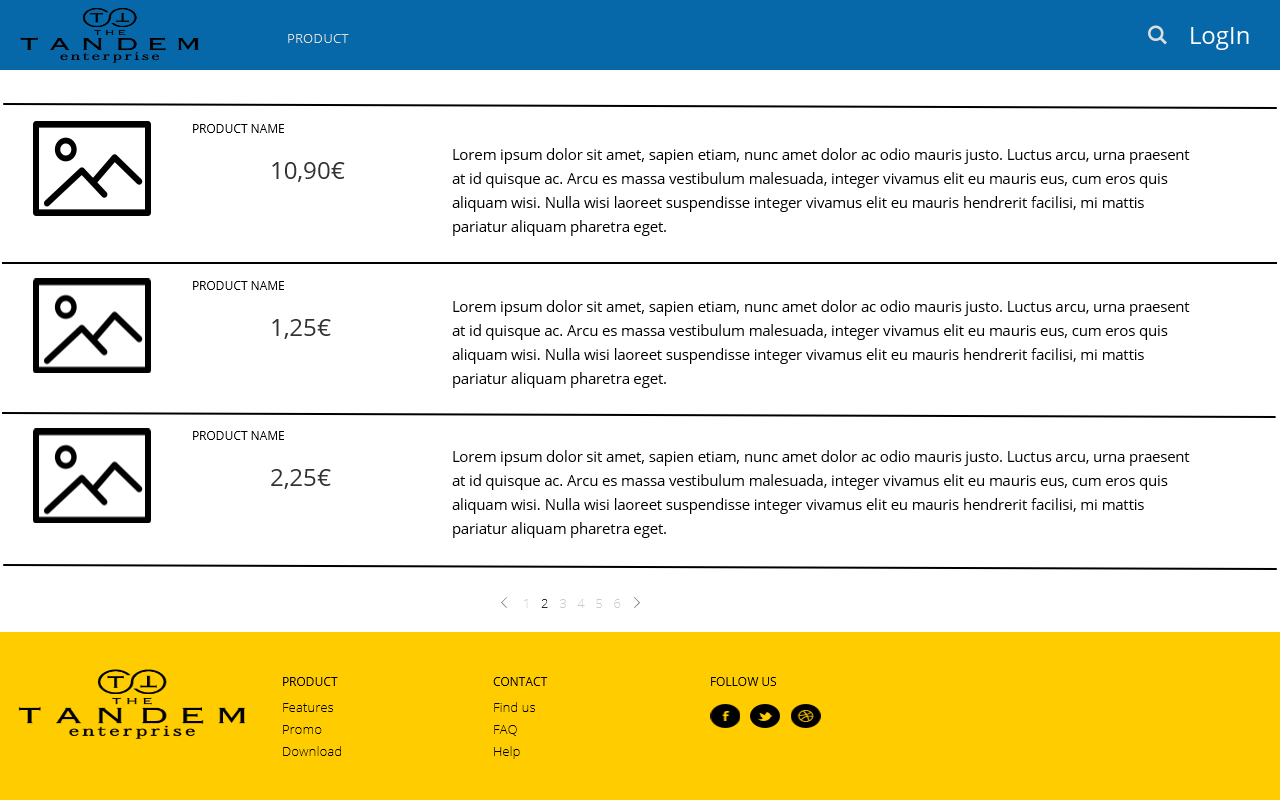
\includegraphics[scale=0.25]{mockup/Inicio.png}
    \caption{Pantalla Principal}
    \label{Fig:Inicio}
\end{figure}
\quad Esta es la pantalla principal, en cada una de las pantallas estarán presentes la barra de navegación con el logo de la empresa y las pestañas, la pestaña de login solo sera visible solo si el usuario no está registrado, si el usuario está registrado se habilitarán otras pestañas que se verán más adelante.
La pestaña de product te llevara a esta misma página y el icono de la lupa puedes buscar un producto.\\
También se mostrara el footer, donde también estarán el logo de la empresa y los contactos.\\
En esta pantalla principal se verán todos los productos disponibles con su nombre, precio y descripción. Si se clickea uno de los productos este te llevara a la propia pantalla de ese producto. 

\begin{figure}[h]
    \centering
    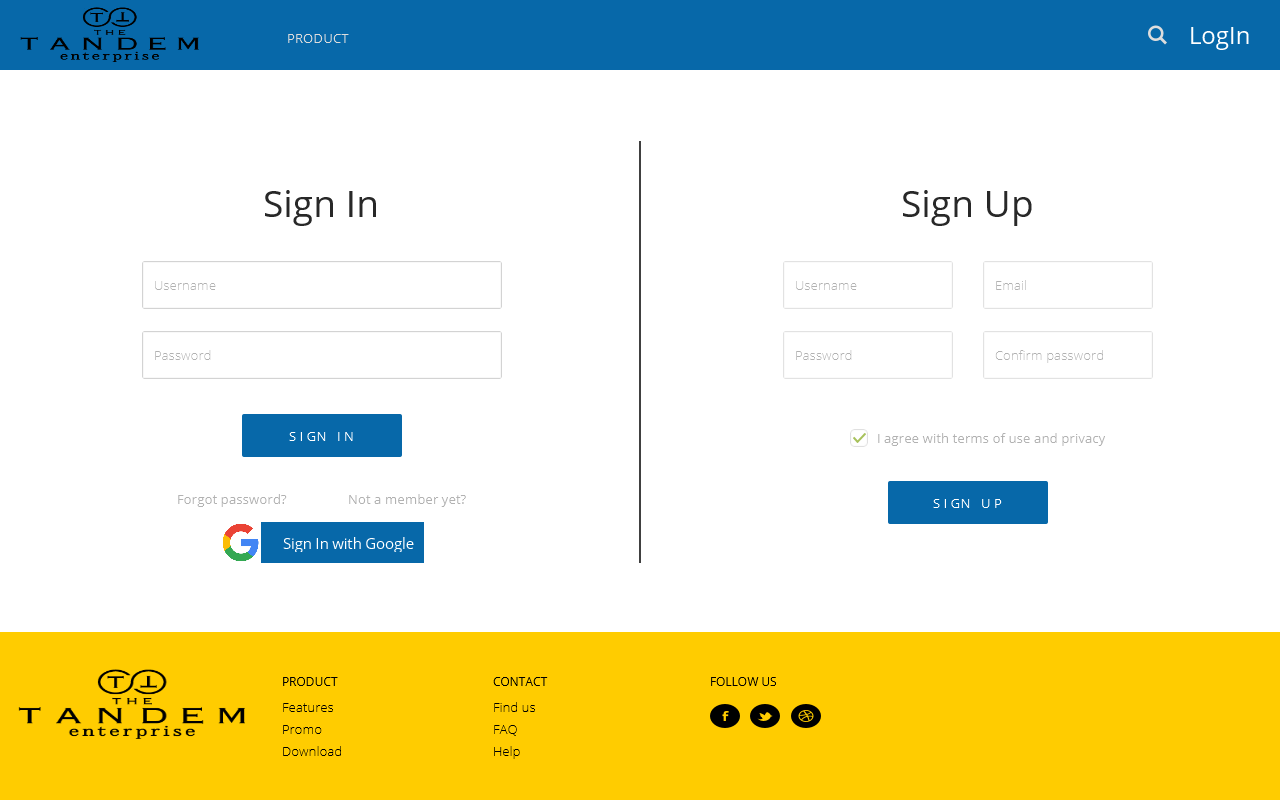
\includegraphics[scale=0.25]{mockup/Login.png}
    \caption{Iniciar sesión/Registrar usuario}
    \label{Fig:Login}
\end{figure}
\quad En esta pantalla el usuario podra iniciar sesión o registrarse.\\
Para iniciar sesión se le pedirá nombre de usuario y contraseña o en su lugar tener una cuenta con google.\\
Para registrarse solo se pedirá nombre de usuario, email, contraseña y que acepte los términos de la empresa, los datos que faltan de la tabla usuario se pedirán a la hora de realizar la compra o el usuario podra rellenarlos en su perfil como veremos más adelante.

\begin{figure}[h]
    \centering
    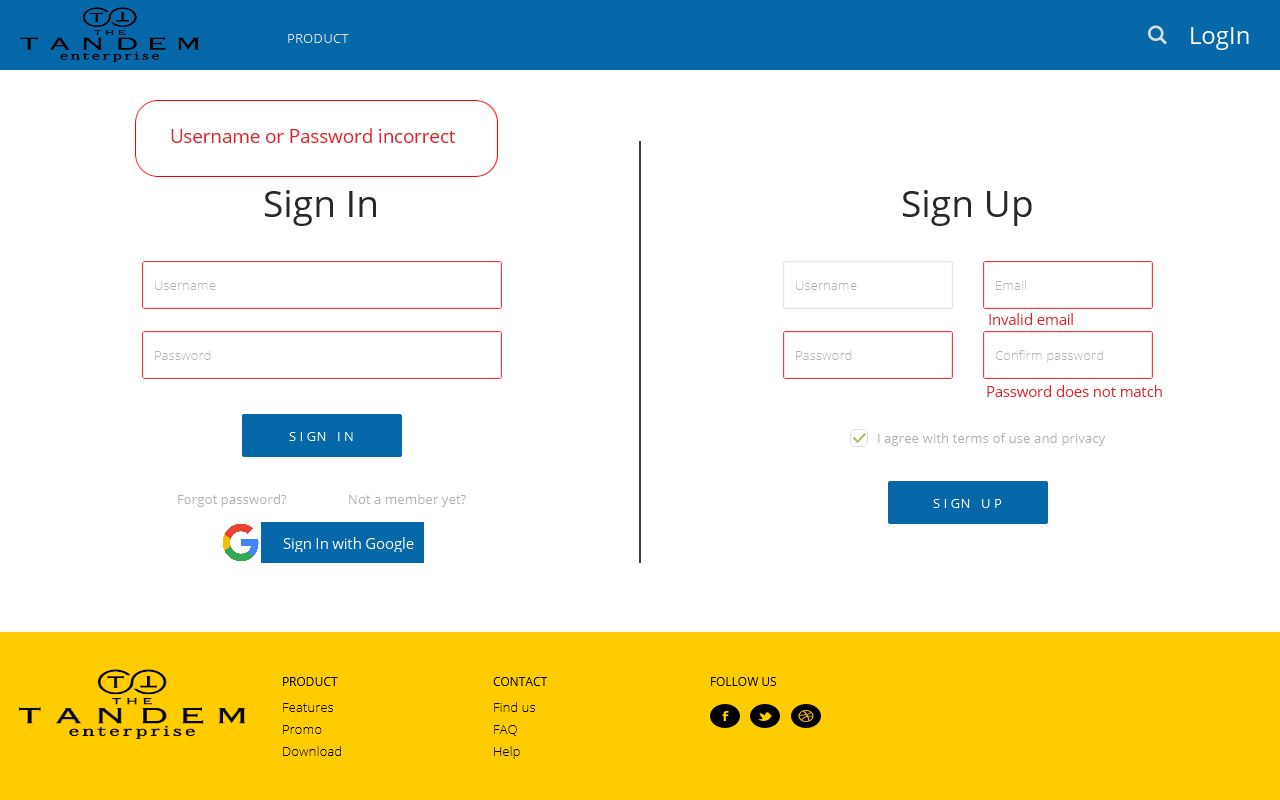
\includegraphics[scale=0.25]{mockup/Fail_login.png}
    \caption{Fallo en Iniciar sesión/Registrar usuario}
    \label{Fig:Fail_login}
\end{figure}
\quad Si el usuario comete algún error se le comunicara con estos avisos y hasta que no los corrija no podra iniciar sesión o registrarse.

\newpage

\begin{figure}[h]
    \centering
    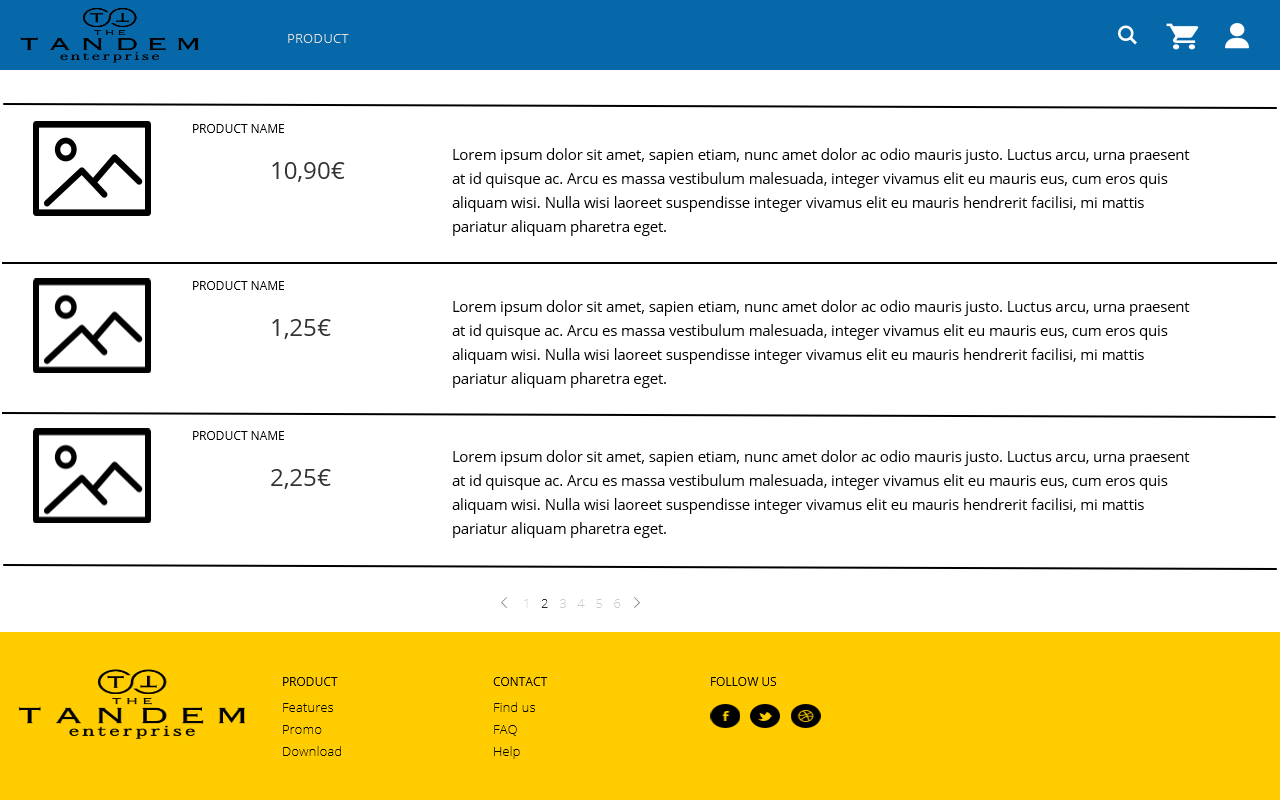
\includegraphics[scale=0.25]{mockup/Inicio_loged.png}
    \caption{Pantalla principal con usuario registrado}
    \label{Fig:Inicio_loged}
\end{figure}
\quad Cuando el usuario inicie sesión volverá a esta pantalla principal, pero ahora en vez de una pestaña login encontraremos el carrito y el perfil del usuario.
\begin{figure}[h]
    \centering
    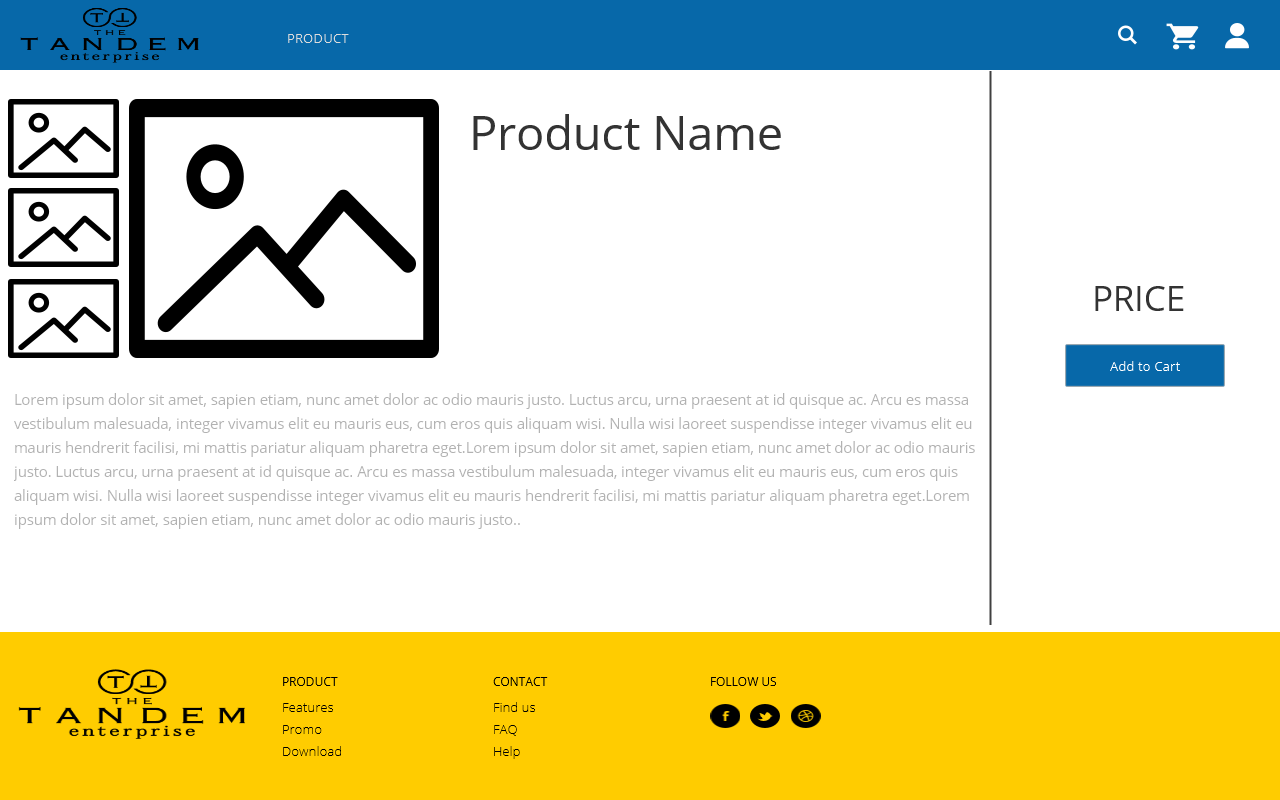
\includegraphics[scale=0.25]{mockup/product_view.png}
    \caption{Pantalla de un producto}
    \label{Fig:product_view}
\end{figure}\\
\quad Cuando el usuario quiera ver un producto le redirigirá a una pantalla de este tipo, en donde podra ver varias imágenes del producto, tendrá una descripción más amplia que en la pantalla principal y podra añadir este producto a la cesta de la compra.

\newpage
\begin{figure}[h]
    \centering
    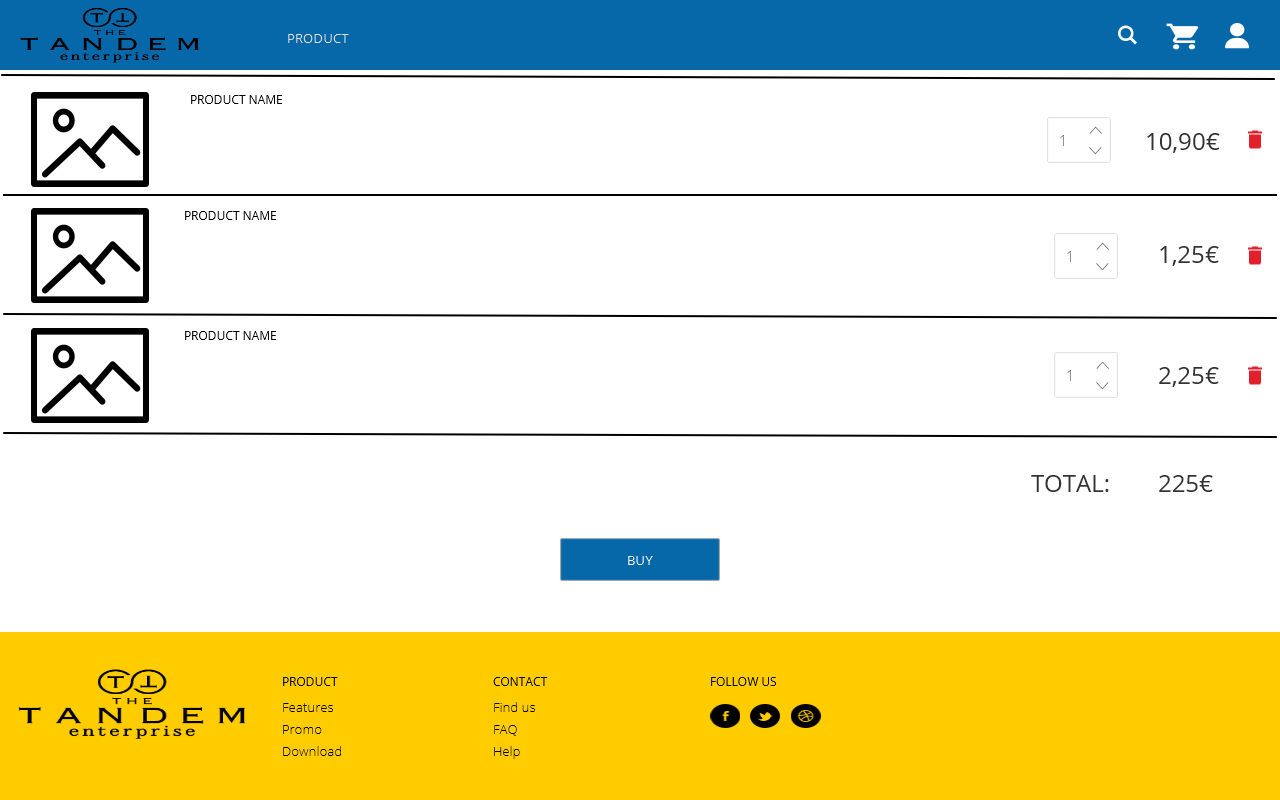
\includegraphics[scale=0.25]{mockup/cart.png}
    \caption{Pantalla del carrito de la compra}
    \label{Fig:cart}
\end{figure}
\quad Esta es la pantalla del carrito, donde el usuario podra ver los productos que ha añadido a su cesta. El usuario podra elegir la cantidad que quiere de cada producto o si quiere eliminarlo de la cesta, también podra ver el precio total de la compra y una vez ya sepa lo que quiere comprar le podra dar al botón correspondiente con esta acción (esta acción no estará implementada en este proyecto por ahora a petición de la empresa).

\begin{figure}[h]
    \centering
    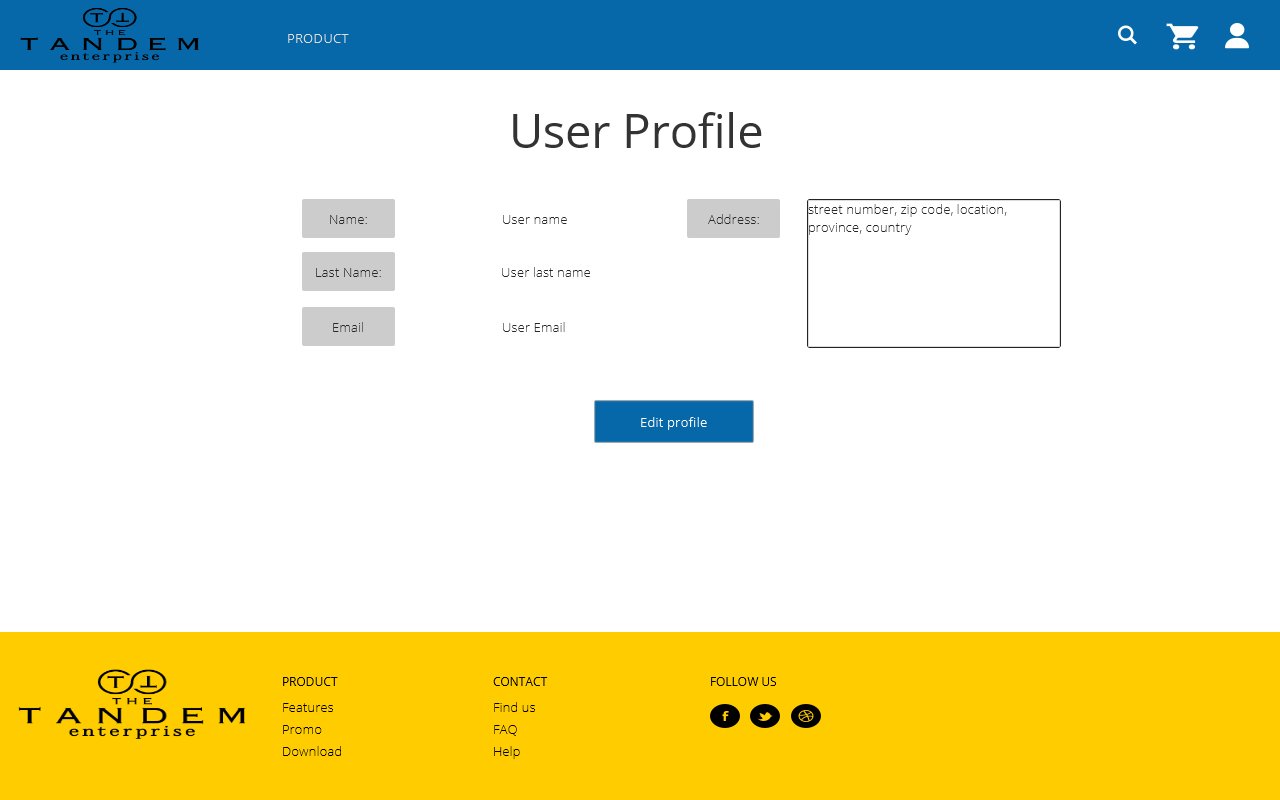
\includegraphics[scale=0.25]{mockup/Profile.png}
    \caption{Pantalla del perfil del usuario}
    \label{Fig:Profile}
\end{figure}
\quad Esta pantalla es donde el usuario podra ver sus datos y si quiere modificar algo le dará al botón de edit profile.

\newpage
\begin{figure}[h]
    \centering
    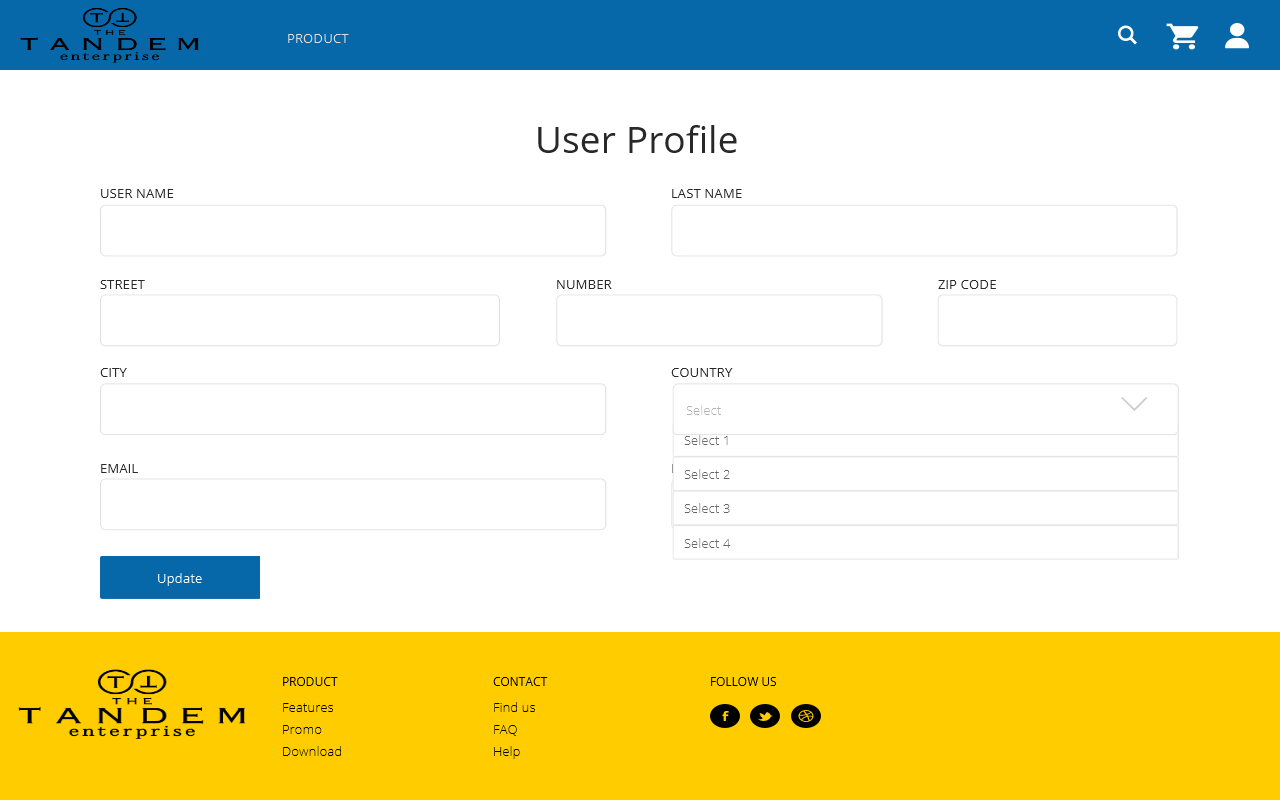
\includegraphics[scale=0.25]{mockup/Update.png}
    \caption{Pantalla para añadir o modificar datos de usuario}
    \label{Fig:Update}
\end{figure}
\quad Cuando el usuario quiera cambiar o añadir datos a su perfil sera redirigido a esta página, donde podra rellenar todos los datos relacionados con el usuario.

\begin{figure}[h]
    \centering
    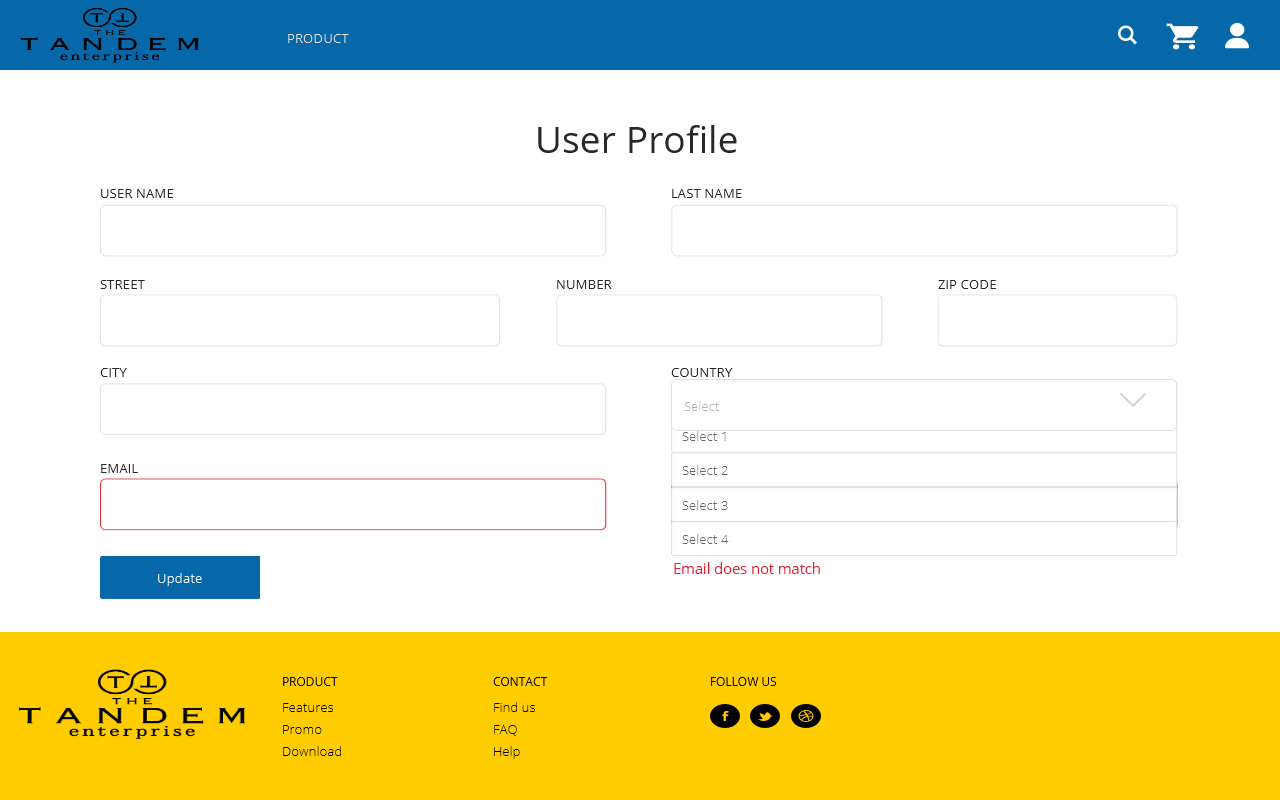
\includegraphics[scale=0.25]{mockup/Fail_update.png}
    \caption{Fallo al añadir o modificar datos de usuario}
    \label{Fig:Fail_update}
\end{figure}
\quad Si el usuario no rellena correctamente estos campos, se le avisara que campos no son correctos para que pueda corregirlos.\\

\begin{center}
    \href{https://github.com/Nestorbd/Full-Stack-Proyect/tree/master/E-commerce/Doncumentation/FullStack_Prototype}{\textbf{\textcolor{blue}{\underline{PROTOTIPO}}}}
\end{center}

\subsection{Usabilidad}
\quad Aqui vamos a ver las caracteristicas basicas de usabilidad que tiene el proyecto:
\begin{itemize}
    \item Facil de aprender e intuitiva \\
   \phantom{ab}Estos dos puntos son complementarios, la pagina web es intuitiva ya que la estructura y funcionamiento son muy parecidos a los que se utilizan en otros sitios web dedicados al comercio como amazon y ebay.
   \begin{figure}[h]
    \ContinuedFloat*
    \centering
    \begin{subfigure}[h]{0.45\textwidth}
    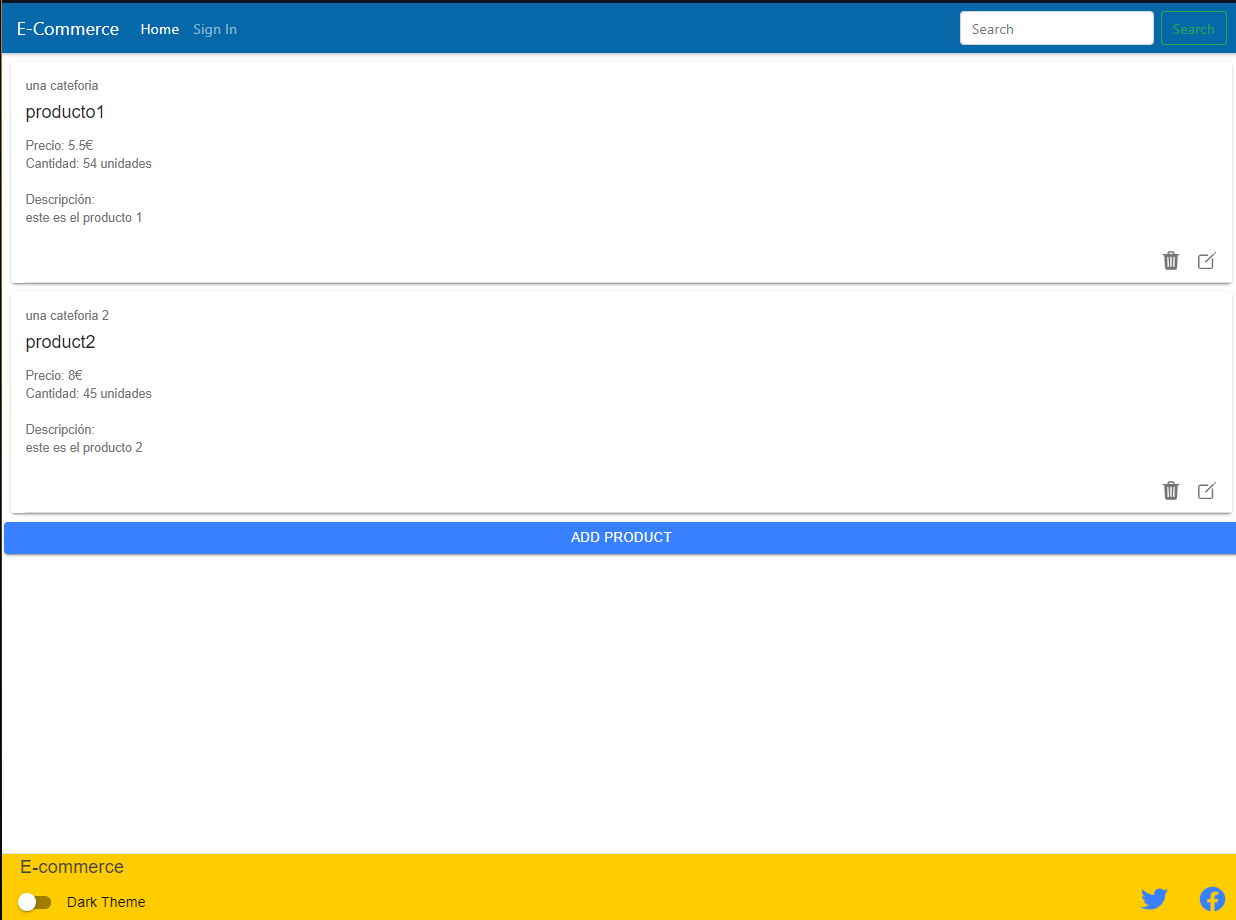
\includegraphics[scale=0.25]{usability/home.png}
    \caption{Vista Principal}
    \label{Fig:Home}
    \end{subfigure}
    
\end{figure} 
   
   \item Previsión de errores\\
   \phantom{ab}Como se ve en las siguientes imagenes se notificara al usuario si algún dato de los que ha introducido es erroneo o ha ocurrido algun error.
\begin{figure}[h]
    \ContinuedFloat
    \centering
    \begin{subfigure}[h]{0.45\textwidth}
    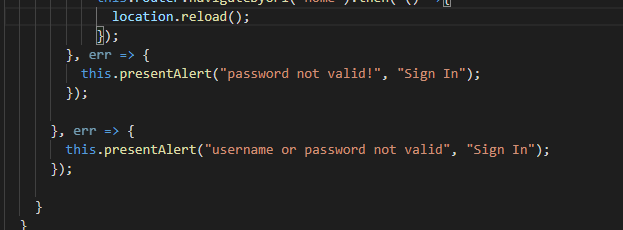
\includegraphics[scale=0.25]{usability/errors.png}
    \caption{Fallo al iniciar sesion}
    \label{Fig:Fail_signIn}
    \end{subfigure}
    \begin{subfigure}[h]{0.45\textwidth}
        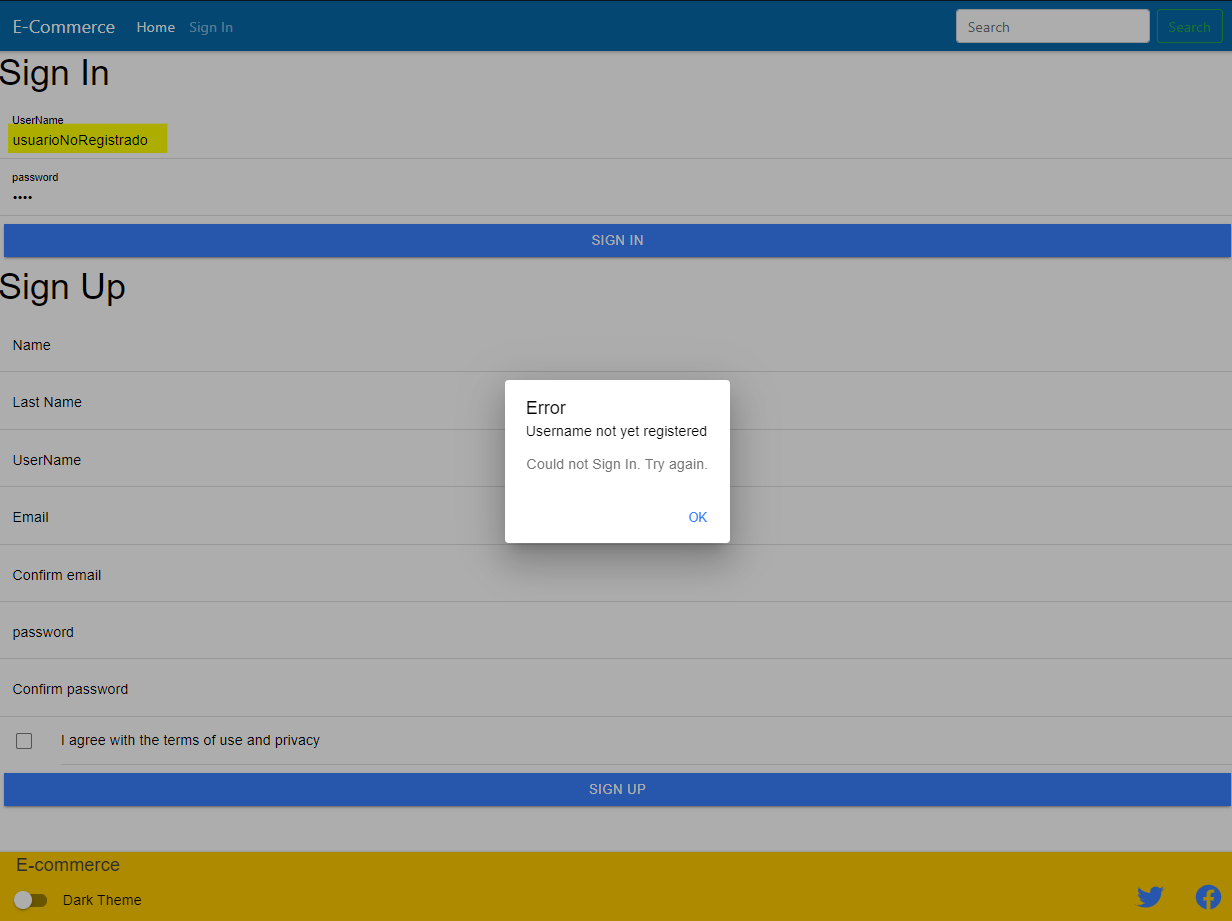
\includegraphics[scale=0.25]{usability/errorWindow.png}
        \caption{Fallo al iniciar sesion}
        \label{Fig:Fail_signIn2}
        \end{subfigure}
\end{figure}
    \item Elegante y simple en su diseño\\
   \phantom{ab}Se usara una paleta de colores basica (amarillo, blanco, azul, negro) basada en la bandera de canarias ya que se usara para vender productos canarios.
   \item Es eficiente\\
   \phantom{ab}Se pide lo que se necesita para el funcionamiento, ni mas ni menos.
   \item Usables
   \begin{itemize}
    \item El usuario es capaz de iniciar acciones y controlarlas, como iniciar y cerrar sesion.
    \item El usuario puede cambiar los colores de la aplicacion, de claro a oscuro, segun su gusto.
    \begin{figure}[h]
        \ContinuedFloat
        \centering
        \begin{subfigure}[h]{0.45\textwidth}
        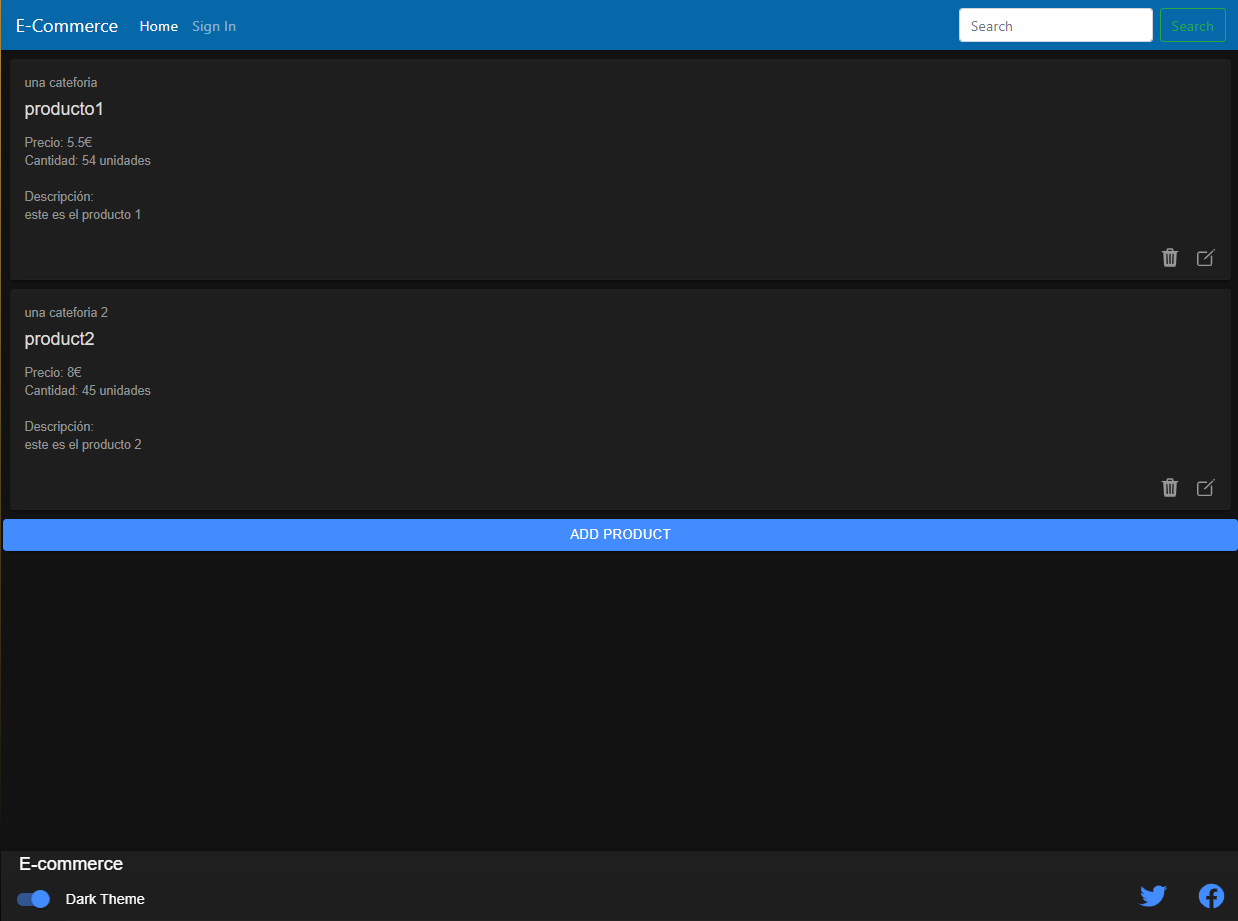
\includegraphics[scale=0.25]{usability/darkTheme.png}
        \caption{Modo Oscuro}
        \label{Fig:DarkTheme}
        \end{subfigure}
        
    \end{figure}
    \item El usuario puede interactuar con la aplicacion y acceder a todo el contenido que se le permite, dependiendo el tipo de usuario que sea.
    \item Si el usuario comete algun error a la hora de insertar datos como por ejemplo en el registro, se le avisara como se hace en la siguiente imagen.
    \begin{figure}[h]
        \ContinuedFloat
        \centering
        \begin{subfigure}[h]{0.45\textwidth}
        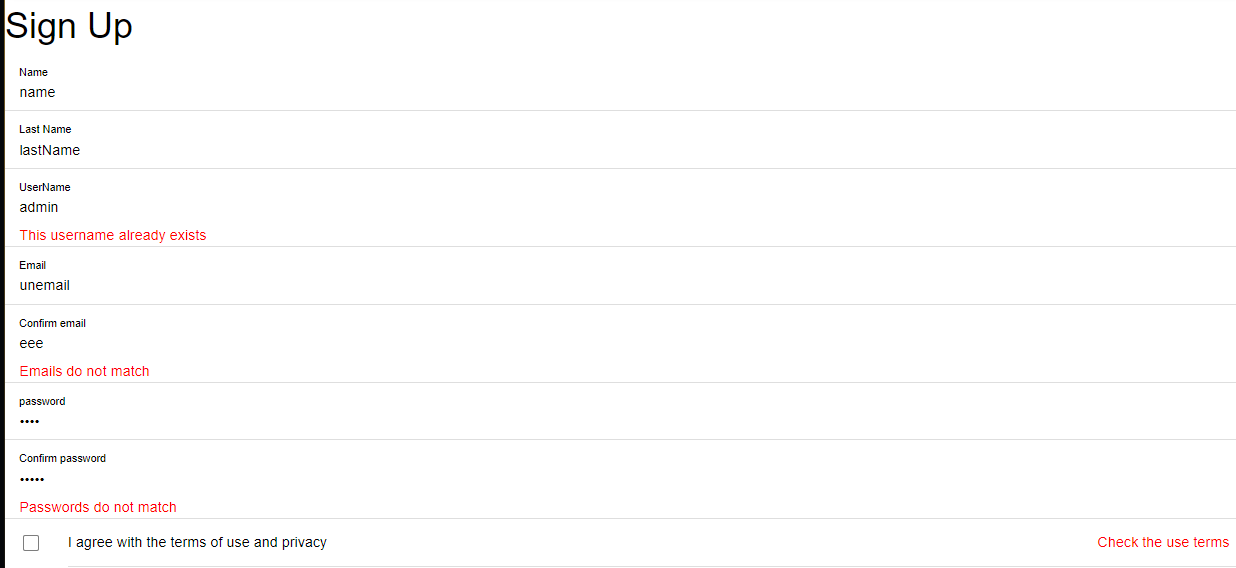
\includegraphics[scale=0.25]{usability/FormsErrors.png}
        \caption{Validacion del formulario}
        \label{Fig:FormsErrors}
        \end{subfigure}
        \begin{subfigure}[h]{0.45\textwidth}
            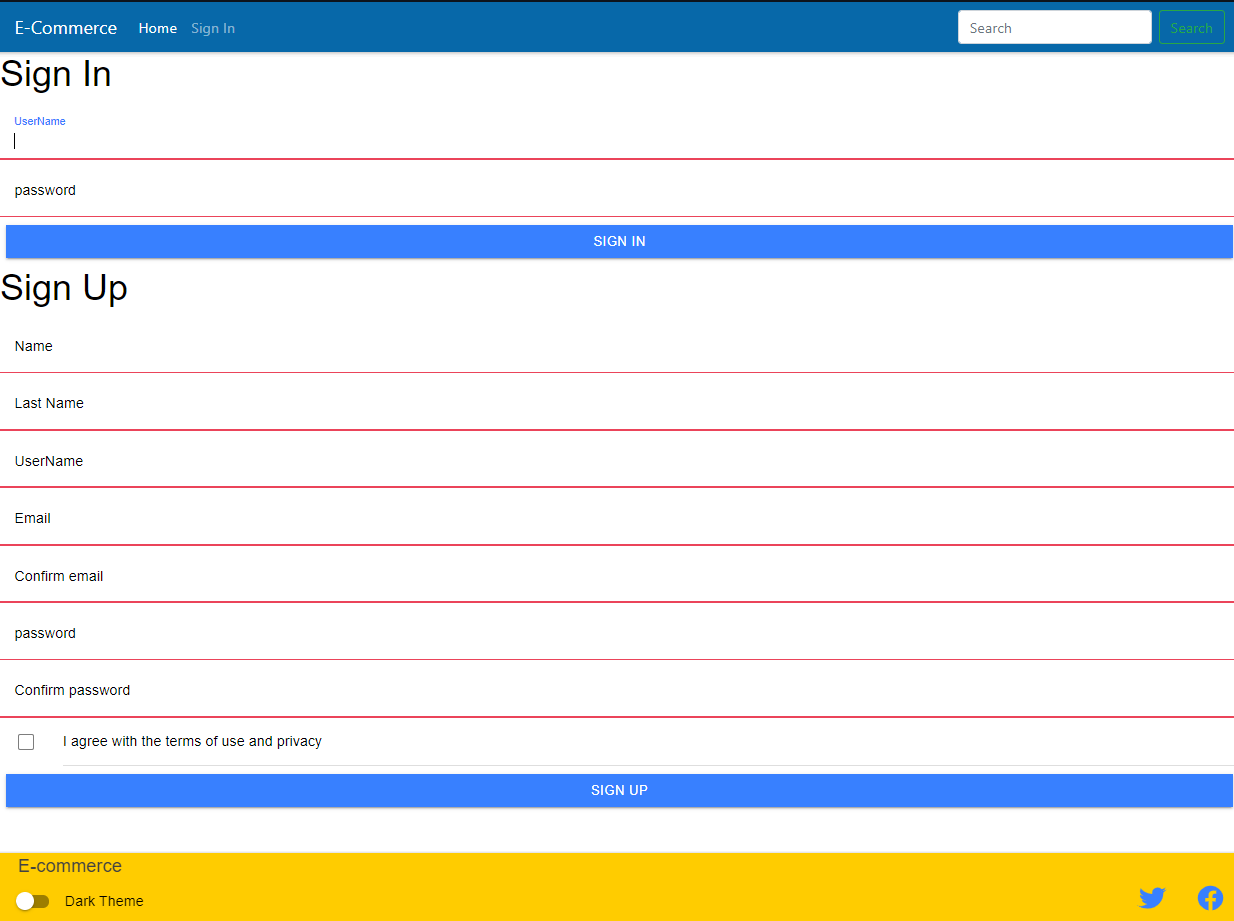
\includegraphics[scale=0.25]{usability/noData.png}
            \caption{Validacion del formulario}
            \label{Fig:FormsErrors2}
            \end{subfigure}
    \end{figure}
   \end{itemize}
   \item Familiaridad del usuario \\
   \phantom{ab}Se puede acceder a la aplicacion desde cualquier dispositivo.
   \item Minima sorpresa \\
   \phantom{ab}El usuario sabra en cada momento que esta haciendo, por lo cual no se llevara ninguna sorpresa.
   \item Seguridad \\
   \phantom{ab}La contraseña del usuario se almacena en la base de datos encriptada con bcrypt y el token codificado en base64.
   \begin{figure}[h]
    \ContinuedFloat
    \centering
    \begin{subfigure}[h]{0.45\textwidth}
    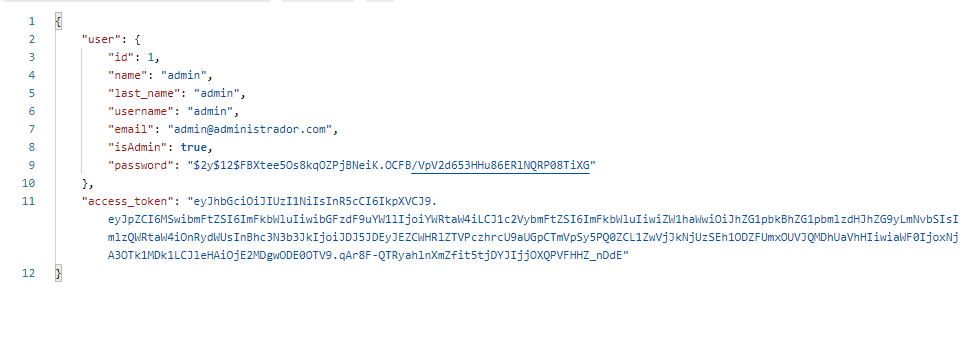
\includegraphics[scale=0.5]{usability/Segurity.png}
    \caption{Encriptacion y codificacion}
    \label{Fig:Security}
    \end{subfigure}
    
\end{figure}
\end{itemize}
\section{Manuales}
\subsection{Instalación para desarrolladores}
\quad Para poder usar la aplicacion primero necesitamos tener instalado las aplicaciones \href{https://git-scm.com/downloads}{\textbf{\textcolor{blue}{Git}}} y \href{https://nodejs.org/es/download/}{\textbf{\textcolor{blue}{node.JS}}}.\\
Despues de tener instalado estas dos aplicaciones tenemos que acceder a una terminal como el cmd en la carpeta en la que se quiere instalar la aplicación y escribir los siguientes comando:\\
\lstset{breaklines=true, basicstyle=\footnotesize}
\begin{lstlisting}[frame=single]
git clone https://github.com/Nestorbd/Full-Stack-Proyect
cd E-commerce/backend
npm install
\end{lstlisting}
Al terminar esto ya tendremos instalado el servidor de la aplicacion.\\
Si quieres que la aplicacion tenga unos datos base necesitaras instalar algun programa como el MySQL Workbench o phpMyAdmin para poder leer el \href{https://github.com/Nestorbd/Full-Stack-Proyect/blob/master/E-commerce/DB_e_comerce.sql}{\textbf{\textcolor{blue}{SQL}}}.\\
Tambien tienes que crear un archivo .env en el backend con los siguientes datos:
\lstset{breaklines=true, basicstyle=\footnotesize}
\begin{lstlisting}[frame=single]
    JWT_SECRET=V3RY#1MP0RT@NT$3CR3T#

    MYSQL_DATABASE=db_e_commerce
    MYSQL_USER=root
    MYSQL_PASSWORD=root
    MYSQL_ROOT_PASSWORD=root
    
    DB_HOST=localhost
    
    NODE_ENV=development
\end{lstlisting}
Para instalar el cliente tenemos que volver al directorio raiz E-commerce y hacer lo siguiente:
\lstset{breaklines=true, basicstyle=\footnotesize}
\begin{lstlisting}[frame=single]
cd E-commerce/frontend/e-commerce
npm install
\end{lstlisting}
Y ya estaria instalado el cliente, ahora para arrancar la aplicacion primero tenemos que arrancar el servidor y luego el cliente, a continuacion explico como se hace.\\
Primero hay que volver al directorio raiz E-commerce y hacer lo siguiente:
\lstset{breaklines=true, basicstyle=\footnotesize}
\begin{lstlisting}[frame=single]
    cd E-commerce/backend
    node server.js
    \end{lstlisting}
Ahora abrimos otra consola en el directorio raiz y hacemos esto:
\lstset{breaklines=true, basicstyle=\footnotesize}
\begin{lstlisting}[frame=single]
    cd E-commerce/frontend/e-commerce
    ionic serve
    \end{lstlisting}
Y listo, ya tenemos nuestra aplicacion instalada y funcionando.
\section{Pila tecnológica}
\begin{itemize}
\item \textbf{Backend:}
\begin{itemize}
\item Node.JS
\item MySQL (BD)
\item Sequelize (ORM)
\end{itemize}
\item \textbf{Frontend:}
    \begin{itemize}
    \item Ionic-Angular
    \end{itemize}
    \item \textbf{Servicio Web:}
    \begin{itemize}
    \item RestFull
    \end{itemize}
\end{itemize}
\section{Comparación de tecnologias}
\subsection{IONIC}
\quad Es un framework que se está haciendo muy popular últimamente. 
Es una herramienta que los programadores pueden utilizar totalmente gratis, 
para desarrollar apps basadas en HTML5, CSS y JavaScript. Está construido con
 Sass y optimizado para AngularJS. Además, es libre y de código abierto, open source.

 \begin{itemize}
   \item \textbf{\underline{Ventajas}}
    \begin{itemize}
\item \textbf{AngularJS}
Trabaja perfectamente con AngularJS. Dando lugar a una arquitectura robusta para el desarrollo de apps. Podrás crear apps móviles ricas y robustas, para colgar en tu tienda de apps favorita.
    \item \textbf{Es fácil de entender}
    No tendrás que complicarte demasiado la vida utilizando el framework, es bastante sencillo de entender. Es desarrollar un código una vez y reutilizarlo las veces que quieras.
    \item \textbf{Pulcro}
    Es moderno y está diseñado para trabajar con lo más actual, con un diseño limpio y pulcro. Los componentes son atractivos, la tipografía, etc.
    \item \textbf{Crea, construye, prueba y compila}
    Podrás crear, construir, y compilar apps en cualquier plataforma, todo con un solo comando. Por eso se considera un potente CLI.
    \item \textbf{Funciona rápido}
    Si te desesperas con poco, te gustará Ionic. Está hecho para ser rápido.
    \item \textbf{Ionic Creator}
    Una de las ventajas de este framwork, es una de sus herramientas, Ionic Creator. Básicamente permite crear las Interfaces sin tener que meter el código a machete. Podrás crear la parte gráfica fácil sin tocar el código para nada.
    \end{itemize}
    \item \textbf{\underline{Desventajas}}
    \begin{itemize}
        \item Es un lenguaje híbrido, nunca va a funcionar tan rápido como una app nativa.
        \item No tiene todas las funcionalidades que puede tener una app nativa.
        \item No es recomendable para proyectos muy grandes.
        \item Puede que algunos componentes te toque programarlos específicamente para iOS.
    \end{itemize}
 \end{itemize}

\section{Repositorios}
\begin{center}
    \href{https://github.com/Nestorbd/Full-Stack-Proyect}{\textbf{\textcolor{blue}{\underline{GitHub}}}}
\end{center}
\section{Planificación}
\quad Planificación hecha con kanban en github: \href{https://github.com/Nestorbd/Full-Stack-Proyect/projects/1}{\textbf{\textcolor{blue}{\underline{link}}}}
\section{Enlaces}

\begin{itemize}
  \item  \href{https://documenter.getpostman.com/view/12915886/TVspjUfE}{\textbf{\textcolor{blue}{\underline{POSTMAN}}}}
\end{itemize}

\end{document}